\documentclass[aspectratio=169, table]{beamer}

\usepackage{array}
\usepackage{colortbl}
\usepackage{tabularx}
\usepackage{xcolor}
\usepackage{tikz}
\usetikzlibrary{arrows.meta, positioning, calc, fit}

\makeatletter
\def\input@path{{../theme/}}
\makeatother
\graphicspath{{../theme/}{../../figures/}}
\usetheme{Pradita}

\newcommand{\sectionframe}[1]{%
  \begin{frame}{\hfill}
    \centering
    \Huge{\textbf{#1}}
  \end{frame}
}

\newcommand{\takeaway}[1]{%
  \vspace{4pt}
  {\footnotesize #1}
}

\title{\huge Lapisan Aplikasi\\
  \vspace{8pt}
  pada ArchiMate}
\subtitle{IT30713 - Enterprise \& Platform Architecture}
\author{\textbf{Alfa Yohannis}}
\date{4 Juli 2026}

\begin{document}

\frame{\titlepage}

\begin{frame}[fragile]
  \frametitle{Contents}
  \vspace{20pt}
  \begin{columns}[t]
    \column{0.5\textwidth}
    \tableofcontents[sections={1-4}]

    \column{0.5\textwidth}
    \tableofcontents[sections={5-8}]
  \end{columns}
\end{frame}

\begin{frame}{\hfill}
  \centering
  \Huge{\textbf{Data sudah dimodelkan---perangkat lunak apa yang mengolahnya?}}
\end{frame}

% ============================================================
\section{Orientasi Bab}
\sectionframe{Orientasi Bab}

\begin{frame}{Tujuan Pembelajaran}
  \vspace{6pt}
  \begin{itemize}
    \item Menjelaskan elemen \textbf{lapisan aplikasi} ArchiMate: komponen,
          layanan, fungsi, dan antarmuka aplikasi.
    \item Menyusun \textbf{application landscape} dan memetakan komponen ke
          layanan bisnis yang diwujudkannya.
    \item Menempatkan analisis dalam \textbf{TOGAF ADM Fase C (Aplikasi)}:
          \emph{baseline}, \emph{target}, dan kesenjangan.
    \item Menautkan aplikasi ke \textbf{data} (akses objek data) dan
          \textbf{bisnis} (realisasi layanan), serta pola integrasi.
  \end{itemize}
  \takeaway{Arah sesi: dari ``data apa'' menuju ``perangkat lunak apa yang
  menjalankan proses \& mengolah data''.}
\end{frame}

\begin{frame}{Ringkasan Awal Bab}
  \vspace{6pt}
  \begin{itemize}
    \item Lapisan aplikasi menutup \textbf{Fase C}: layanan aplikasi
          \emph{mewujudkan} layanan bisnis \& \emph{melayani} proses bisnis.
    \item \textbf{Fungsi aplikasi mengakses objek data}---di sinilah akses data
          langsung berada (bukan pada proses bisnis).
    \item Studi kasus berjalan: lanskap \textbf{API-led} rel Transfer
          Dana---gateway, aplikasi transfer, AML, adaptor BI-FAST, rekonsiliasi.
    \item Keluaran bab memperkuat \textbf{Analisis} domain aplikasi makalah.
  \end{itemize}
  \takeaway{Lapisan aplikasi menutup rantai keterlacakan: motivasi $\rightarrow$
  bisnis $\rightarrow$ aplikasi $\rightarrow$ data.}
\end{frame}

% ============================================================
\section{Mengapa Lapisan Aplikasi}
\sectionframe{Mengapa Lapisan Aplikasi}

\begin{frame}{Posisi Lapisan Aplikasi dalam ArchiMate}
  \vspace{2pt}
  \centering
  \scalebox{0.74}{
    \begin{tikzpicture}[
      font=\small\bfseries,
      node distance=2.2mm,
      layer/.style={draw, rounded corners=1.5mm, align=left, minimum width=82mm,
        minimum height=10mm, inner xsep=4mm},
      strat/.style={layer, fill=orange!16},
      biz/.style={layer, fill=praditagreen!22},
      app/.style={layer, fill=blue!26, draw=blue!70!black, line width=0.6mm},
      tech/.style={layer, fill=gray!18},
      impl/.style={layer, fill=orange!10},
    ]
      \node[strat] (s) {STRATEGI\\
        \footnotesize\mdseries Sumber daya, kapabilitas, arah tindakan};
      \node[biz, below=of s] (b) {BISNIS\\
        \footnotesize\mdseries Aktor, peran, proses, layanan, objek bisnis};
      \node[app, below=of b] (a) {APLIKASI \quad$\leftarrow$ \emph{fokus sesi ini}\\
        \footnotesize\mdseries \textbf{Komponen, layanan, fungsi, antarmuka}, objek data};
      \node[tech, below=of a] (t) {TEKNOLOGI (\& FISIK)\\
        \footnotesize\mdseries Node, perangkat, jaringan, \emph{system software}};
      \node[impl, below=of t] (i) {IMPLEMENTASI \& MIGRASI\\
        \footnotesize\mdseries \emph{Work package}, \emph{deliverable}, \emph{gap}};
      \node[draw, rounded corners=2mm, fill=purple!22, align=center,
        text width=16mm, minimum height=60mm, right=5mm of a, font=\bfseries]
        (mot) {M\\O\\T\\I\\V\\A\\S\\I\\[2mm]\footnotesize\mdseries (mengapa)};
    \end{tikzpicture}
  }

  \takeaway{Komponen aplikasi \emph{menggelar} perilaku yang mewujudkan layanan
  bisnis; dipetakan ke fase \textbf{C (Sistem Informasi)} TOGAF ADM.}
\end{frame}

\begin{frame}{Tiga Pola Integrasi Aplikasi}
  \vspace{4pt}
  \centering
  \scalebox{1.12}{
    \begin{tikzpicture}[
      font=\small,
      lbl/.style={font=\small\bfseries},
      app/.style={circle, draw=blue!70!black, fill=blue!10, minimum size=8.5mm, inner sep=0pt},
      hub/.style={rectangle, rounded corners=1mm, draw=orange!80!black, fill=orange!16, minimum width=14mm, minimum height=8mm},
      gw/.style={rectangle, rounded corners=1mm, draw=praditagreen, fill=praditagreen!14, minimum width=16mm, minimum height=8mm},
      lnk/.style={draw=gray!55}
    ]
      \node[lbl] at (1.4,3.6) {Titik-ke-titik};
      \foreach \a/\x/\y in {a/0/2.6, b/2.8/2.6, c/0/0.8, d/2.8/0.8, e/1.4/1.7} \node[app] (\a) at (\x,\y) {};
      \foreach \p/\q in {a/b,a/c,a/d,a/e,b/c,b/d,b/e,c/d,c/e,d/e} \draw[lnk] (\p)--(\q);
      \node[lbl] at (5.9,3.6) {Hub / ESB};
      \node[hub] (h) at (5.9,1.7) {\textbf{ESB}};
      \foreach \a/\x/\y in {h1/4.6/2.6, h2/7.2/2.6, h3/4.6/0.8, h4/7.2/0.8} {\node[app] (\a) at (\x,\y) {}; \draw[lnk] (\a)--(h);}
      \node[lbl] at (10.4,3.6) {API-led};
      \node[app] (ext) at (10.4,2.6) {};
      \node[gw] (g) at (10.4,1.6) {\textbf{Gateway}};
      \foreach \a/\x in {p1/9.2, p2/10.4, p3/11.6} {\node[app] (\a) at (\x,0.6) {}; \draw[lnk] (g)--(\a);}
      \draw[lnk] (ext)--(g);
    \end{tikzpicture}
  }

  \takeaway{Rel transfer memakai \textbf{API-led} lewat gateway: aman, terkelola,
  dan sejalan dengan ``API sebagai produk''.}
\end{frame}

% ============================================================
\section{TOGAF ADM Fase C}
\sectionframe{TOGAF ADM Fase C:\\ Arsitektur Aplikasi}

\begin{frame}{Siklus TOGAF ADM}
  \vspace{8pt}
  \begin{columns}[c]
    \column{0.4\textwidth}
    \centering
    \scalebox{0.85}{
      \begin{tikzpicture}[
        font=\footnotesize\bfseries,
        phase/.style={circle, draw=praditagreen, line width=0.4mm,
          fill=praditagreen!15, minimum size=11mm, inner sep=0pt},
        reqman/.style={circle, draw=blueColor, line width=0.4mm, fill=blueColor!15,
          minimum size=21mm, inner sep=1pt, align=center, font=\scriptsize\bfseries},
        prelim/.style={circle, draw=orange!80!black, line width=0.4mm,
          fill=orange!25, minimum size=13mm, inner sep=0pt, align=center,
          font=\scriptsize\bfseries},
        ring/.style={-Latex, draw=praditagreen!75, line width=0.4mm},
        spoke/.style={draw=blueColor!35, line width=0.25mm},
      ]
        \node[reqman] (rm) at (0,0) {Manajemen\\Requirements};
        \foreach \ang/\lab in {90/A, 45/B, 0/C, -45/D, -90/E, -135/F, 180/G, 135/H}
          \node[phase] (\lab) at (\ang:2.6cm) {\lab};
        \node[prelim] (P) at (90:4.1cm) {Prelim.};
        \foreach \lab in {A,B,C,D,E,F,G,H} \draw[spoke] (\lab) -- (rm);
        \foreach \a/\b in {A/B, B/C, C/D, D/E, E/F, F/G, G/H, H/A}
          \draw[ring] (\a) to[bend left=12] (\b);
        \draw[ring, draw=orange!80!black] (P) -- (A);
        \node[phase, fill=blue!45, line width=0.7mm] at (0:2.6cm) {C};
      \end{tikzpicture}
    }
    \column{0.6\textwidth}
    {\footnotesize TOGAF (\emph{The Open Group Architecture Framework}); ADM
    (\emph{Architecture Development Method}).\par}
    \vspace{5pt}
    \footnotesize
    \begin{itemize}\setlength{\itemsep}{1.0pt}
      \item \textbf{Prelim.}---Persiapan \& prinsip
      \item \textbf{A}---Visi Arsitektur
      \item \textbf{B}---Arsitektur Bisnis
      \item \textbf{\textcolor{blue!70!black}{C---Arsitektur Sistem Informasi
            (Data \& Aplikasi)}} $\leftarrow$ \emph{sesi ini (Aplikasi)}
      \item \textbf{D}---Arsitektur Teknologi
      \item \textbf{E}---Peluang \& Solusi
      \item \textbf{F}---Perencanaan Migrasi
      \item \textbf{G}---Tata Kelola Implementasi
      \item \textbf{H}---Manajemen Perubahan Arsitektur
      \item \textbf{Manajemen Requirements}---di pusat
    \end{itemize}
  \end{columns}
\end{frame}

\begin{frame}{Fase C (Aplikasi): Lima Langkah}
  \vspace{2pt}
  \footnotesize
  \begin{columns}[t]
    \column{0.5\textwidth}
    \textbf{Apa \& Mengapa}
    \begin{itemize}\setlength{\itemsep}{2.5pt}
      \item Sisi \textbf{Aplikasi} Fase C: perangkat lunak yang mewujudkan
            layanan bisnis dan mengolah data.
      \item Menghasilkan \emph{application landscape} \textbf{baseline} \&
            \textbf{target}.
      \item Selisihnya = \textbf{analisis kesenjangan}.
    \end{itemize}
    \column{0.5\textwidth}
    \textbf{Lima Langkah}
    \begin{enumerate}\setlength{\itemsep}{2.5pt}
      \item Ruang lingkup \& prinsip aplikasi.
      \item Lanskap aplikasi \textbf{baseline}.
      \item Lanskap aplikasi \textbf{target}.
      \item Analisis \textbf{kesenjangan}.
      \item Masukan ke Fase D (teknologi).
    \end{enumerate}
  \end{columns}
  \vspace{2pt}
  \takeaway{Keluaran: katalog komponen/layanan, diagram kerja sama aplikasi, dan
  matriks komponen--fungsi bisnis.}
\end{frame}

% ============================================================
\section{Elemen Lapisan Aplikasi}
\sectionframe{Elemen Lapisan Aplikasi}

\begin{frame}{Jenis Elemen dan Simbolnya di Archi}
  \vspace{6pt}
  \begin{columns}[c]
    \column{0.56\textwidth}
    \centering
    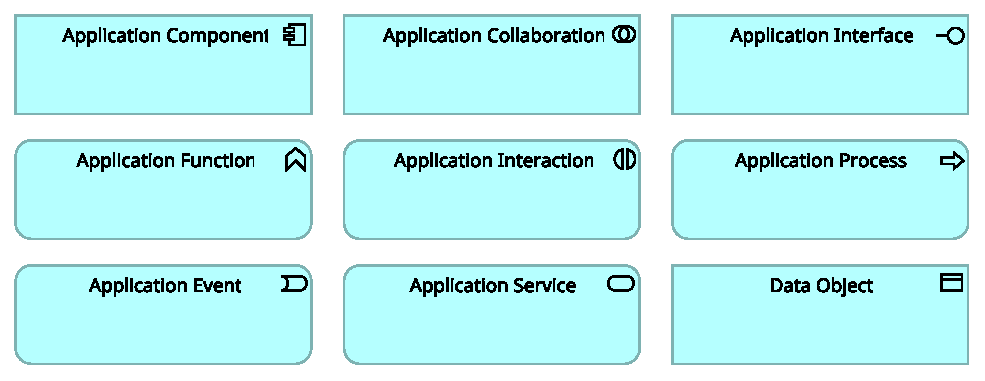
\includegraphics[width=\linewidth]{app-legend.pdf}
    \column{0.44\textwidth}
    \footnotesize
    \begin{itemize}\setlength{\itemsep}{3pt}
      \item \textbf{Komponen} -- perangkat lunak yang digelar.
      \item \textbf{Layanan} -- yang ditawarkan komponen.
      \item \textbf{Fungsi} -- perilaku internal; mengakses data.
      \item \textbf{Antarmuka} -- titik akses (REST API).
      \item \textbf{Objek data} -- struktur pasif (Bab 6).
    \end{itemize}
  \end{columns}
  \takeaway{Elemen aplikasi berwarna kebiruan; ikon pojok membedakan jenisnya.}
\end{frame}

\begin{frame}{Membedakan Elemen Aplikasi}
  \vspace{6pt}
  \begin{itemize}
    \item \textbf{Layanan (service):} apa yang ditawarkan---``Layanan API
          Transfer''; \emph{mewujudkan} layanan bisnis.
    \item \textbf{Fungsi (function):} perilaku internal---``Eksekusi
          Pembayaran''; \emph{mengakses} objek data.
    \item \textbf{Komponen (component):} perangkat lunak---``API Gateway'',
          ``Mesin AML''.
    \item \textbf{Antarmuka (interface):} titik akses---``REST API (SNAP BI)''.
  \end{itemize}
  \takeaway{Satu komponen menjalankan banyak fungsi \& menawarkan banyak layanan;
  satu layanan dipakai banyak proses.}
\end{frame}

\begin{frame}{}
  \centering
  \vspace{1mm}
  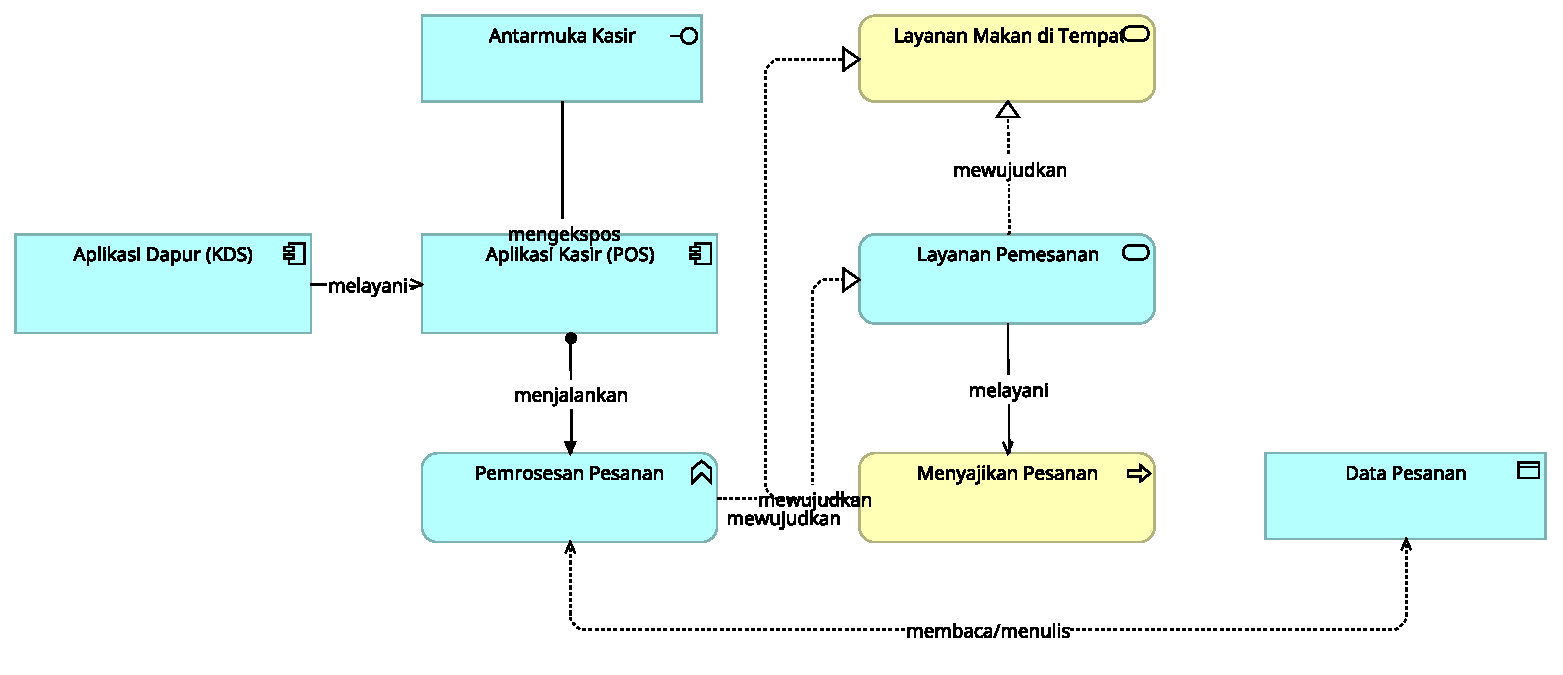
\includegraphics[width=\textwidth,height=.8\textheight,keepaspectratio]{app-contoh.pdf}\\
  {\scriptsize Contoh interaksi antar-elemen aplikasi (kasus restoran): komponen
  menjalankan fungsi, fungsi mewujudkan layanan \& mengakses data.}
\end{frame}

% ============================================================
\section{Studi Kasus: Aplikasi di Archi}
\sectionframe{Studi Kasus:\\ Arsitektur Aplikasi Transfer di Archi}

\begin{frame}{}
  \centering
  \vspace{1mm}
  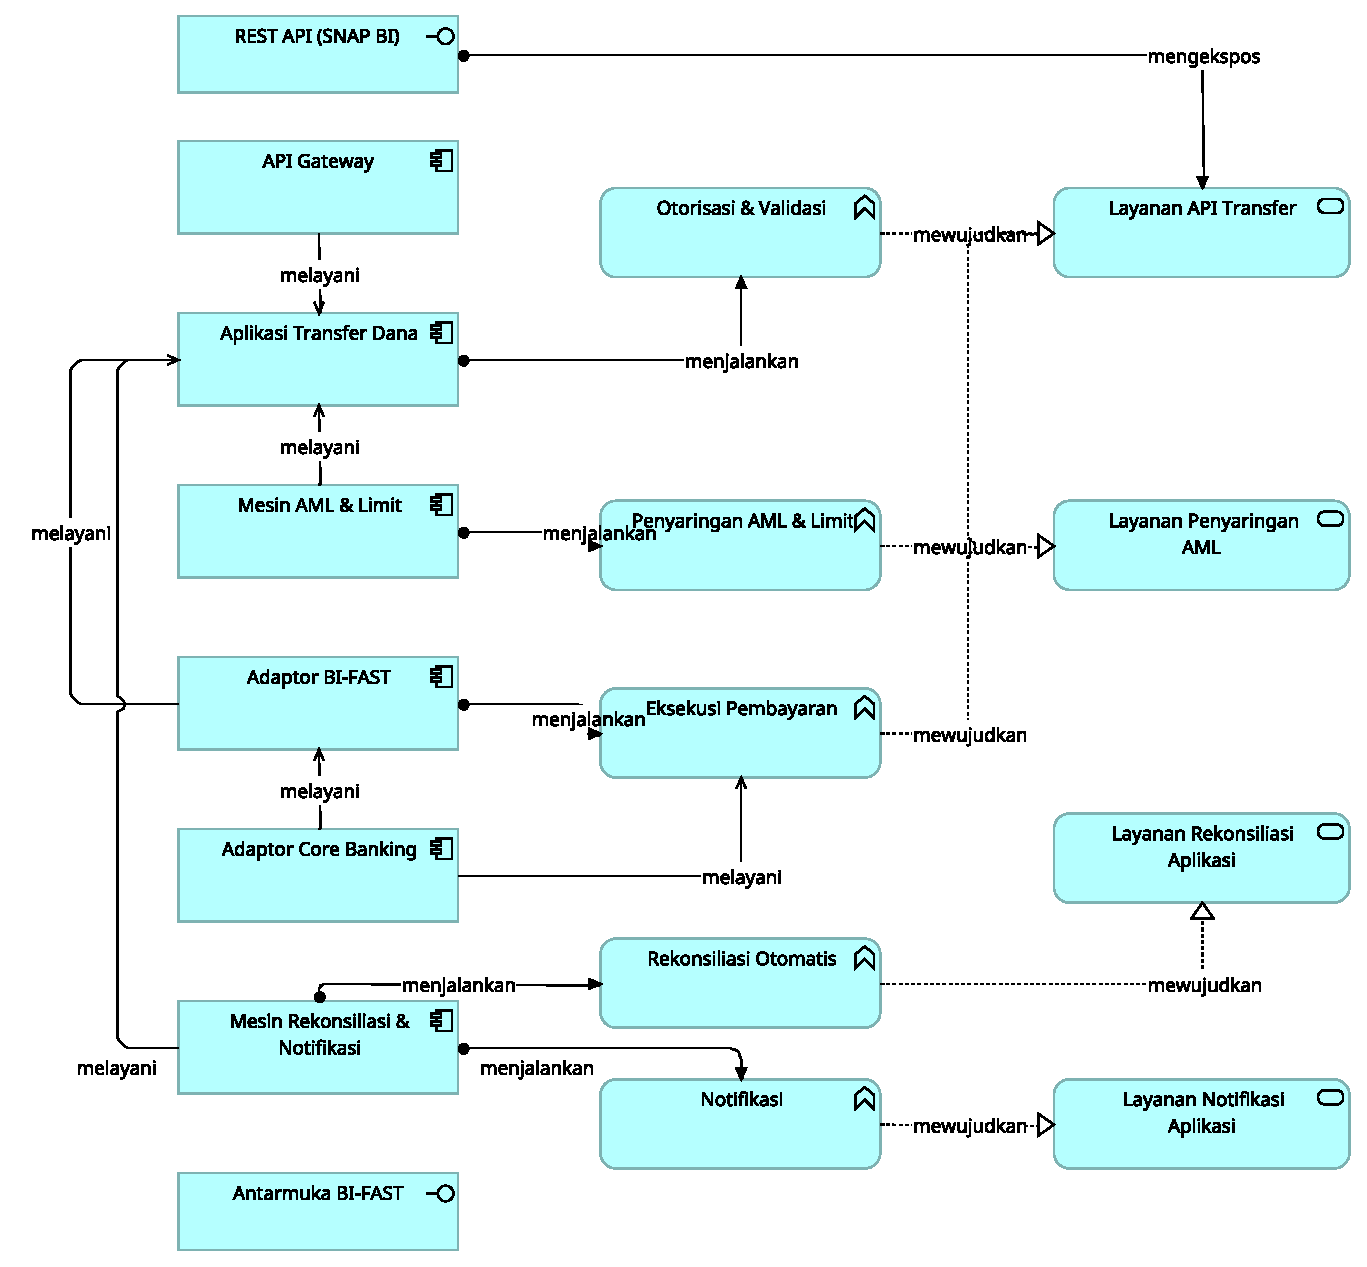
\includegraphics[width=\textwidth,height=.84\textheight,keepaspectratio]{app-transfer.pdf}\\
  {\scriptsize Lanskap aplikasi: komponen \emph{menjalankan} fungsi, fungsi
  \emph{mewujudkan} layanan aplikasi, antarmuka \emph{mengekspos}, komponen saling \emph{melayani}.}
\end{frame}

\begin{frame}{}
  \centering
  \vspace{1mm}
  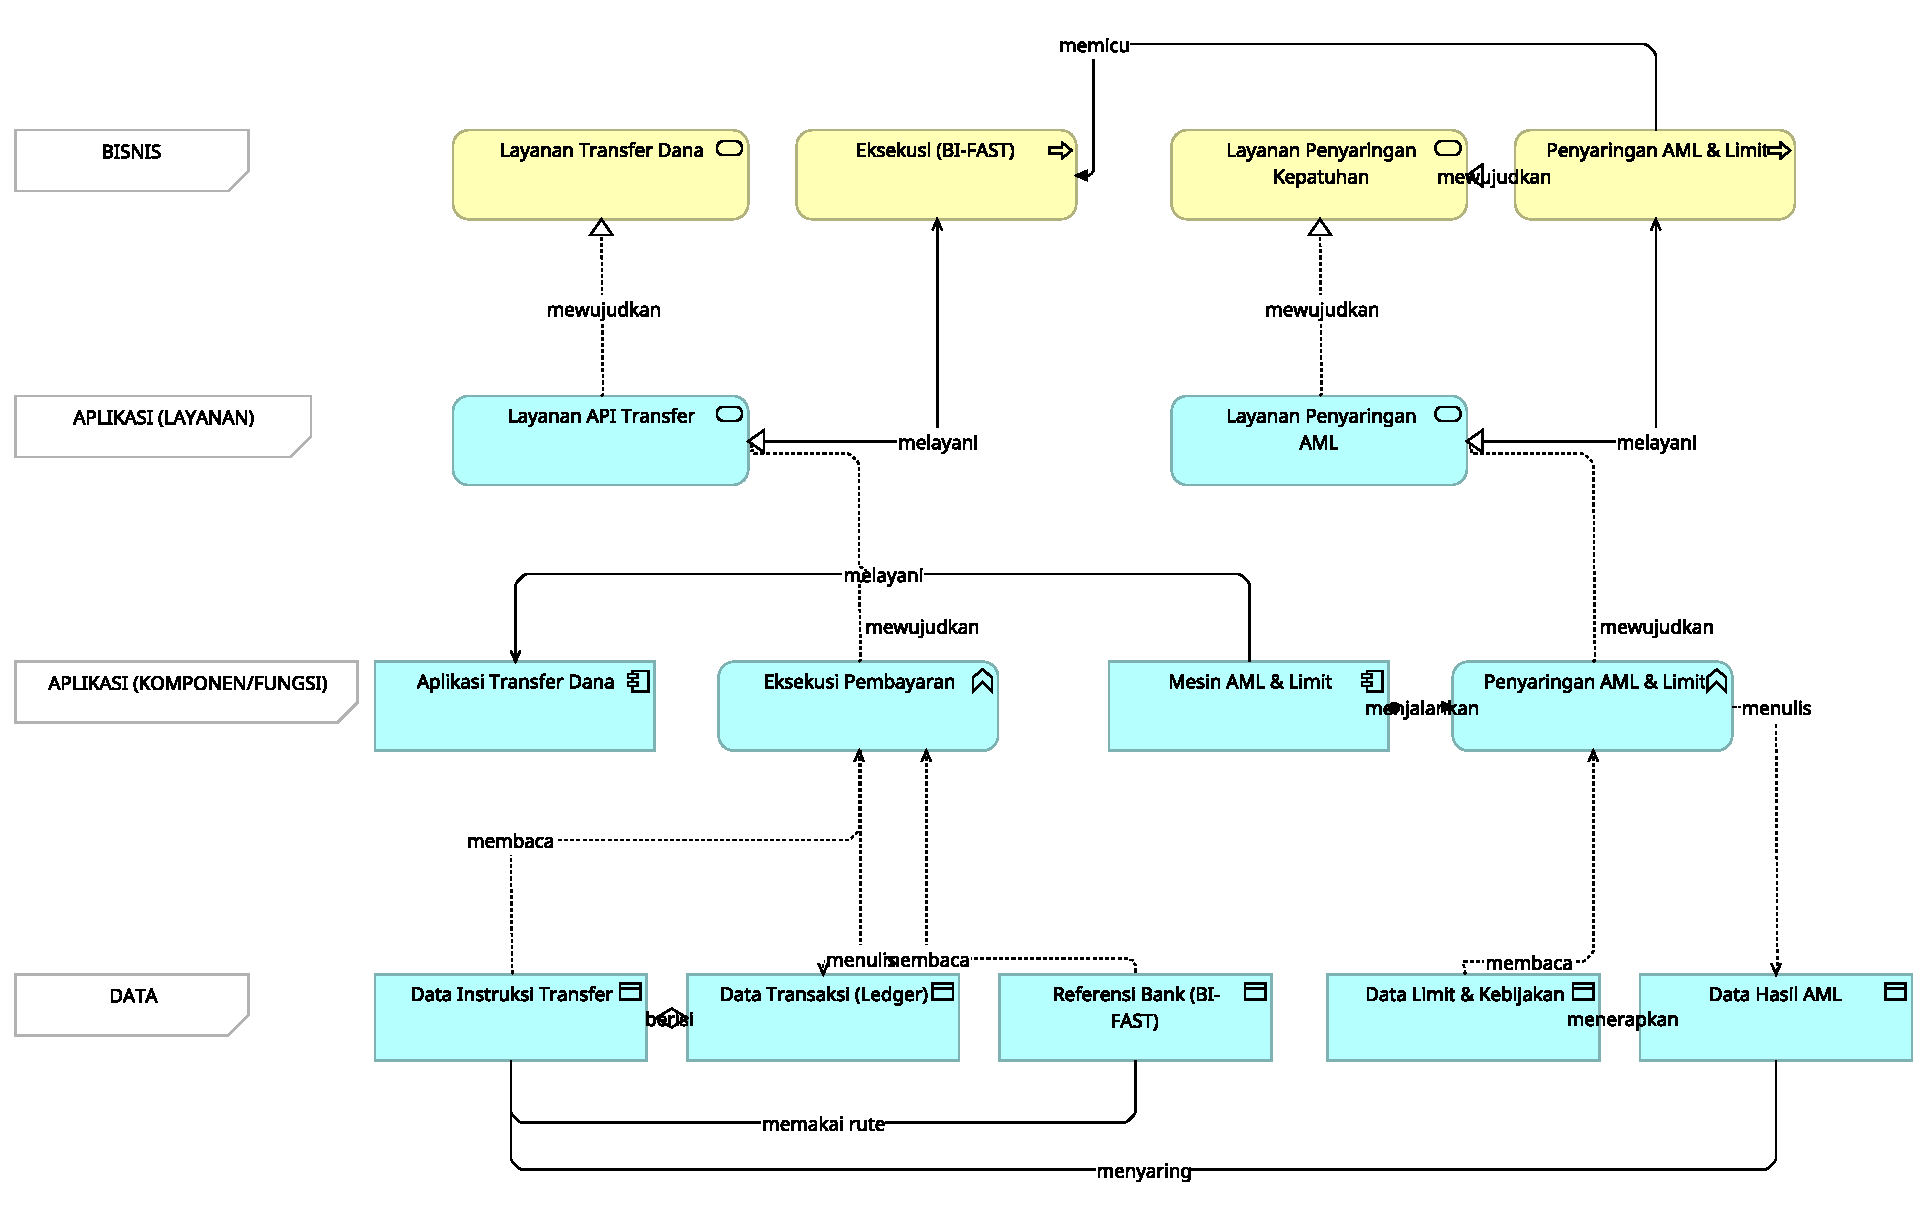
\includegraphics[width=\textwidth,height=.84\textheight,keepaspectratio]{app-stack.pdf}\\
  {\scriptsize Penyelarasan \textbf{Bisnis--Aplikasi--Data}: layanan aplikasi
  mewujudkan layanan bisnis \& melayani proses; fungsi aplikasi \emph{mengakses} objek data.}
\end{frame}

\begin{frame}{Cara Membaca: Rantai Lengkap Fase C}
  \vspace{4pt}
  \footnotesize
  \begin{itemize}\setlength{\itemsep}{2.5pt}
    \item \textbf{Realisasi:} Layanan API Transfer \emph{mewujudkan} Layanan
          Transfer Dana (bisnis); fungsi \emph{mewujudkan} layanan aplikasi.
    \item \textbf{Serving:} layanan aplikasi \emph{melayani} proses bisnis;
          komponen saling melayani.
    \item \textbf{Assignment:} komponen \emph{menjalankan} fungsi aplikasi.
    \item \textbf{Access:} \textbf{fungsi aplikasi} \emph{membaca}/\emph{menulis}
          objek data---akses data langsung ada di sini.
  \end{itemize}
  \takeaway{Rantai keterlacakan tertutup: proses bisnis $\leftarrow$ layanan
  aplikasi $\leftarrow$ fungsi $\rightarrow$ objek data.}
\end{frame}

% ============================================================
\section{Latihan dan Jembatan}
\sectionframe{Latihan dan Jembatan}

\begin{frame}{Latihan Terapan Individual}
  \vspace{8pt}
  \begin{itemize}
    \item \textbf{Latihan 7.1} -- Lanskap aplikasi (komponen, fungsi, layanan,
          antarmuka + ketergantungan).
    \item \textbf{Latihan 7.2} -- Penyelarasan lintas-lapisan (bisnis--aplikasi--
          data) untuk satu kapabilitas.
    \item \textbf{Latihan 7.3} -- Pola integrasi \& baseline--target.
    \item \textbf{Latihan 7.4} -- Paragraf analisis aplikasi.
  \end{itemize}
  \takeaway{Semua latihan menjadi bahan langsung Analisis domain aplikasi
  makalah.}
\end{frame}

\begin{frame}{Jembatan ke Bab Berikutnya}
  \vspace{8pt}
  \begin{itemize}
    \item Bab berikutnya turun ke \textbf{lapisan teknologi}: node, perangkat,
          jaringan, dan \emph{system software} yang menggelar komponen.
    \item Artifact pada teknologi \emph{mewujudkan} objek data; node
          \emph{menggelar} komponen aplikasi.
    \item Katalog komponen \& diagram penyelarasan menjadi masukan memilih
          platform dan pola penggelaran.
  \end{itemize}
  \takeaway{Lanskap aplikasi yang jelas adalah fondasi bagi arsitektur teknologi
  dan implementasi.}
\end{frame}

\begin{frame}{\hfill}
  \centering
  \Huge{\textbf{Terima kasih}}\\[8pt]
  \normalsize Pertanyaan \& diskusi
\end{frame}

\end{document}
